\documentclass{article}%
\usepackage[T1]{fontenc}%
\usepackage[utf8]{inputenc}%
\usepackage{lmodern}%
\usepackage{textcomp}%
\usepackage{lastpage}%
\usepackage{authblk}%
\usepackage{graphicx}%
%
\title{Functional EF{-}Hands in Neuronal Calcium Sensor GCAP2 Determine Its Phosphorylation State and Subcellular Distribution In Vivo and Are Essential for Photoreceptor Cell Integrity}%
\author{Karen Jones}%
\affil{Neurophysiology Laboratory, Department of Pharmacology and Experimental Neuroscience, University of Nebraska Medical Center, Omaha, Nebraska, United States of America}%
\date{01{-}01{-}2014}%
%
\begin{document}%
\normalsize%
\maketitle%
\section{Abstract}%
\label{sec:Abstract}%
Studies indicate that Phosphorylation of any number of biological processes in the body may provide clues to early detection of some types of breast cancer, but often these signals arent detected.\newline%
Now, a team of researchers from UT Southwestern Medical Center and the Salk Institute for Biological Studies has found that Phosphorylation of p52A protein 1, which can act as an ion{-}channel jumper and potentially disrupt cancer cell growth, is associated with a key metabolic event in breast cancer that underlies fibrosis and tumor recurrence. They hypothesized that a cellular signaling trigger known as an aphosphorylation of p52A was the primary triggering event that led to the disease progression and tissue atrophy in breast cancer.\newline%
Marilyn Oby, MD, PhD, a scientist in the department of Molecular Pharmacology and the senior author of the study, says, We found that p52A activation was associated with progression and recurrence in breast cancer cells. Our study, which has been published in the journal Cell, shows a link between p52A activity and cell signaling signals promoting tumors and excellent breast cancer recurrence and so{-}called ll clustering of carcinomas.\newline%
The findings are groundbreaking because they reveal that the essential role of p52A in cancer growth and progression isnt going away. The researchers also speculate that this activation process could be traced back to the first source of cellular signaling, possibly peptide therapy.\newline%
While breast cancer is the most common cancer in the United States, women diagnosed in their 20s are five times more likely to die from the disease than women diagnosed in their 50s.\newline%
With average life expectancy among women age 50 to 79, the challenge is to cure this disease and avoid both breast and lung cancer. Before hormone therapy is developed to treat breast cancer, which can take several years to reach its peak efficacy, researchers say, its necessary to find new therapies that have the ability to significantly impact breast cancer spread and recurrence.\newline%
In the study, Oby and her colleagues evaluated the first study in which direct proteomicsa technology that puts breast cancer cell lines through several analysis methods at oncewas used to examine the effects of p52A activation in normal women who had received an estrogen receptor{-}positive breast cancer biopsy. The second study in which a UC San Diego{-}led consortium of researchers from the University of California, San Diego, and UCSF studied the effects of p52A activation on breast cancer cells and appeared to elicit apoptosis in highly active metastatic breast cancer. The third study in which Oby and her colleagues from both collaborating groups conducted a single, non{-}invasive, early{-}detection study in healthy women without invasive breast cancer showed evidence of a relationship between p52A activation and advanced breast cancer tissue atrophy and tumor recurrence.\newline%
Our breakthroughs this work reflects in a field that still uses single studies only show associations, says Oby. This is a valuable lead, as biology is based on multi{-}variable relationships. These relationships tell us something about how proteins work and what factors contribute to the pathogenesis of any disease and how to use those discoveries to improve precision medicine.\newline%
The research was funded by the National Institutes of Health, the Merck Foundation and the Jules Rosen Institute of Biotechnology.

%
\subsection{Image Analysis}%
\label{subsec:ImageAnalysis}%


\begin{figure}[h!]%
\centering%
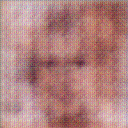
\includegraphics[width=150px]{500_fake_images/samples_5_128.png}%
\caption{A Black And White Photo Of A Black And White Photo}%
\end{figure}

%
\end{document}